\documentclass{article}
\usepackage{amsmath}
\usepackage{amssymb}
\newcommand*{\qed}{\hfill\ensuremath{\blacksquare}}
\newcommand\tab[1][1cm]{\hspace*{#1}}
\usepackage{graphicx}
\graphicspath{{.}}

\title{Computational Linear Algebra, Module 9 (1-10)}
\author{Maya Shende}
\date{Due: March 28st, 2017}

\begin{document}
\maketitle

\begin{enumerate}

%exercise 1
\item Yes, this does draw the function $g(x) = x-\frac{5}{3}x^3$

%exercise 2
\item When more terms are added to the approximation function, we see that it looks like the sine function

%exercise 3
\item 
Errors for interval $[0, 2\pi]:$\\
\begin{tabular}{|c|c|}
	\hline
	n=3	&44.03945\\
	n=5 	&38.71829\\
	n=7	&18.99292\\
	n=13	&0.22859\\	
	\hline
\end{tabular}
The difference between $n=3$ and $n=13$ is $44.03945-0.22859 = 43.81086$. The errors for $n=3$ and $n=13$ for the interval $[0,\pi]$ are: $n=3 \rightarrow 1.13981$ and $n=13 \rightarrow 4.30594 \times 10^{-6}$\\

For the interval $[0, \pi/2]$, the errors are $n=3 \rightarrow 0.01836$ and $n=13 \rightarrow 4.30594 \times 10^{-11}$\\

The error at each point is multiplied by deltaX because we are calculating the area between the two curves to find the error. 

%exercise 4
\item Taylor series expansion: $\sin{x} = x - \frac{x^3}{3!} + \frac{x^5}{5!} - \frac{x^7}{7!} + \frac{x^9}{9!} - \dots$. The coefficients printed in the alpha array are the same as those we saw in the earlier exercise. 

%exercise 5
\item $k=3$: \\
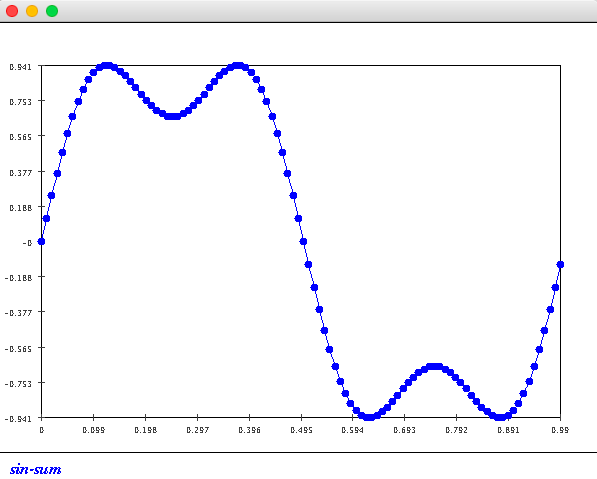
\includegraphics[scale=0.3]{exercise5_k3}\\
$k=5$:\\
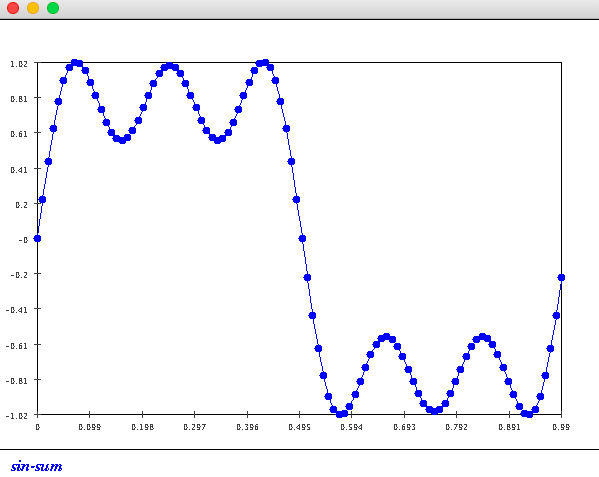
\includegraphics[scale=0.3]{exercise5_k5}\\
$k=7$:\\
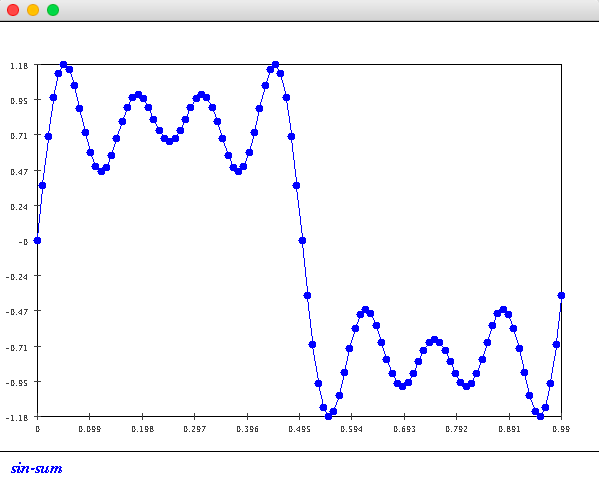
\includegraphics[scale=0.3]{exercise5_k7}\\
$k=9$:\\
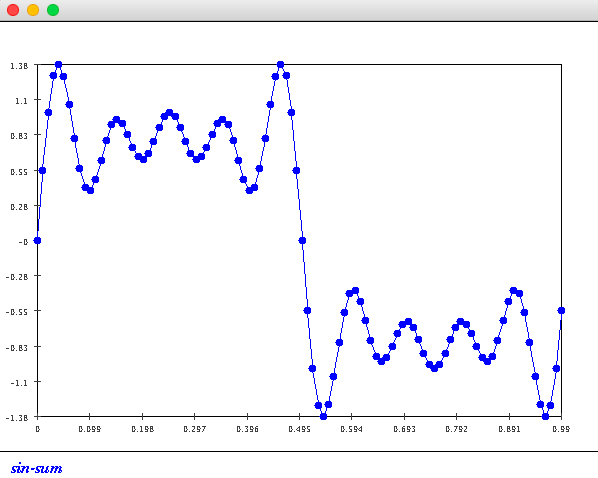
\includegraphics[scale=0.3]{exercise5_k9}\\
$k=11$:\\
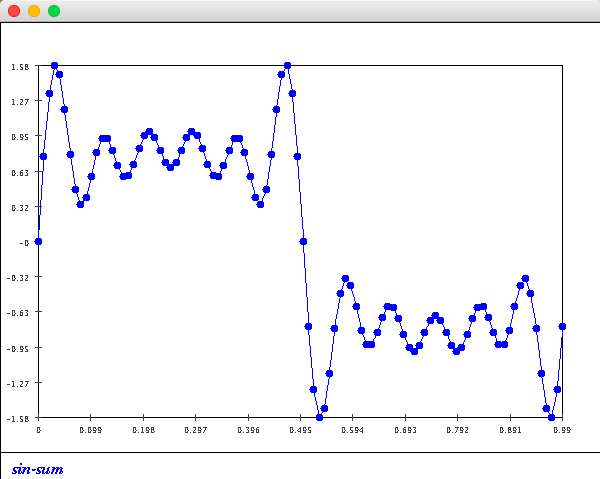
\includegraphics[scale=0.3]{exercise5_k11}\\

%exercise 6
\item Any piecewise function cannot be represented by a linear combination of $\sin{(2\pi kx)}$. For example, 

$ h(x) = $
$ \begin{cases} 
      1 & x\leq 0 \\
      3& 0\leq x\leq 20 \\
      5 & x > 20
   \end{cases}
$

%exercise 7
\item The second graph that is output by this program is a subsection of the first graph, and this is a fractal so the subsection looks like the full graph.

%exercise 8
\item $k=0 \rightarrow$ evaluates to 1\\
$k=1 \rightarrow$ evaluates to $n$\\
$k=n-1 \rightarrow$ evaluates to $n$, which is the same as when $k=1$\\
$k=n \rightarrow$ evaluates to 1, which is the same as when $k=0$

%exercise 9
\item ${n\choose k} = \frac{n!}{k! (n-k)!} \rightarrow$ this is derived by taking the total number of combinations possible, and dividing out the repeated combinations.\\
\begin{tabular}{|c|c|}
	\hline
	k	& ${n\choose k}$\\
	\hline
	0	& 1\\
	\hline
	1	& 5\\
	\hline
	2	& 10\\
	\hline
	3	& 10\\
	\hline
	4	& 5\\
	\hline
	5	& 1\\
	\hline
\end{tabular}

%exercise 10
\item We know that ${n\choose k} = \frac{n!}{k!(n-k)!}$, ${n-1\choose k} = \frac{(n-1)!}{k!(n-1-k)!}$ and ${n-1\choose k-1} = \frac{(n-1)!}{(k-1)!(n-k)!}$. So now we have:
\begin{eqnarray*}
	{n-1\choose k} + {n-1\choose k-1} &=& \frac{(n-1)!}{k!(n-1-k)!} + \frac{(n-1)!}{(k-1)!(n-k)!}\\
	&=& \frac{(n-1)!(n-k) + k(n-1)!}{k!(n-k)!}\\
	&=& \frac{n! - k(n-1)! + k(n-1)!}{k!(n-k)!}\\
	&=& \frac{n!}{k!(n-k)!}\\
	&=& {n\choose k} 
\end{eqnarray*} 
Therefore, ${n\choose k} = {n-1\choose k} + {n-1\choose k-1}$ \qed

$n\choose k$ is a symmetric function because of how choosing combinations works. Pascal's Triangle:\\
\begin{tabular}{ccccccccc}
	\hfill	&\hfill	&\hfill	& \hfill 	& 1	&\hfill	&\hfill	&\hfill	&\hfill\\
	\hfill	&\hfill	&\hfill	&1	& \hfill	& 1	& \hfill	&\hfill	&\hfill\\
	\hfill	&\hfill	&1	&\hfill	&2	&\hfill	&1	&\hfill	&\hfill\\
	\hfill	&1	&\hfill	&3	&\hfill	&3	&\hfill	&1	&\hfill\\
	1	&\hfill	&4	&\hfill	&6	&\hfill	&4	&\hfill	&1
\end{tabular}

Each row of Pascal's Triangle gives the values of $n\choose k$, where k is the column of the row and n is the row number. 

\end{enumerate}
\end{document}